\section{Speichern und Audio}

Die Ausgabe der gewünschten Audio-Dateien wird mit einem sogenannten Körperschallaktor umgesetzt welcher in Abbildung \ref*{fig:schallaktorAdafruit} ersichtlich ist. Dieser ermöglicht es, die ausgesendeten Schwingungen über den Schädelknochen weiterzuleiten. Dadurch kann das Mittelohr umgangen werden und die Hygiene verbessert werden, da kein direkter Kontakt mit dem Gehörgang stattfindet. Für den Bau eines Prototyps wird ein Körperschallaktor des Herstellers Adafruit verwendet. 

\begin{figure}[H]
\begin{center}
	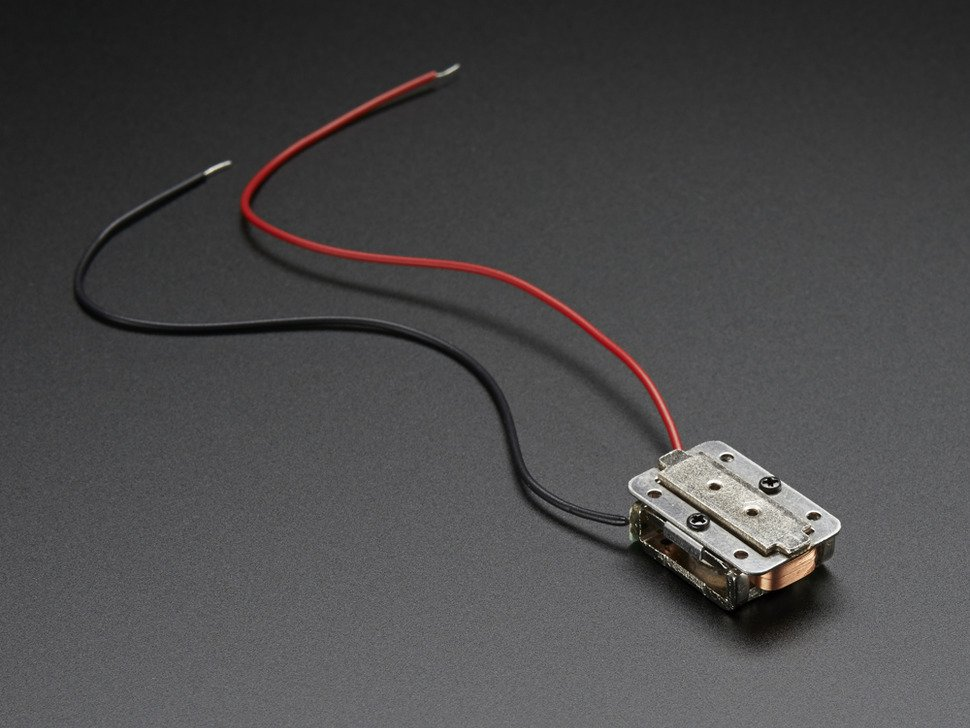
\includegraphics[width=110mm]{data/Schallaktor.png}
	\caption{Körperschallaktor von Adafruit}
	\label{fig:schallaktorAdafruit}
\end{center}
\end{figure}

Das Ziel ist es, bei möglichst geringem Energieverbrauch, eine möglichst intensive Lautstärke, bei guter Audioqualität zu erzielen.
Die Steuerung und Ausgabe der verschiedenen Audiosignale wird von einem zentralen Mikrocontroller übernommen. Ausserdem muss das Audiosignal verstärkt werden. Damit der Energieverbrauch möglichst gering bleibt, wird die Verstärkerstufe wenn möglich digital umgesetzt. Dadurch kann die Anzahl der analogen Bauelemente verringert werden und somit auch der Platzbedarf klein gehalten werden. Als Verstärkerstufe dient der Stereo-Amplifier MAX 98306 oder ein Mono-Amplifier mit ähnlichen Eigenschaften, da nur ein Kanal als Ausgang benötigt wird. Als maximale Ausgangswerte gelten folgende RMS-Referenzwerte: Ein Ausgangsstrom von 150 mA und eine Ausgangspspannung von 750 mV.
Der Leistungsverbrauch der Verstärkereinheit ergibt sich aus den folgenden gemessenen Werten:

\begin{itemize}
\item Strom = 65 mA
\item Spannung = 3,3 V
\end{itemize}
Daraus ergibt sich eine Leistung von 214,5 mW.

Die Speichereinheit wird mit einer externen SD-Karte umgesetzt, die dann manuell entfernt und beschrieben werden kann. Das bedeutet auch, dass die Platzierung der SD-Karte möglichst elegant am Gehäuse erfolgen muss. Zur Aktualisierung kann das Konzept eines prinzipiellen SD-Karten-Hubs, gemäss Abbildung \ref{fig:sdKartenHub} verwendet werden. Dadurch werden mehrere SD-Karten parallel aktualisiert.

\begin{figure}[H]
\begin{center}
	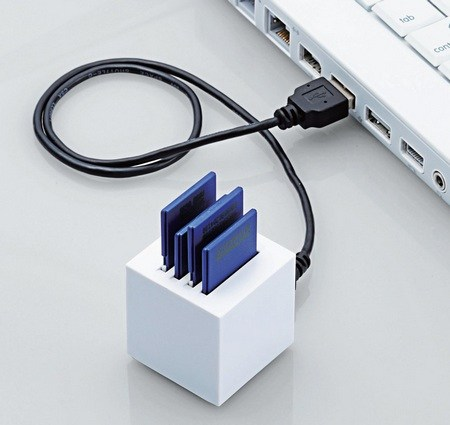
\includegraphics[scale = 0.4]{data/SDKartenHub}
	\caption{SD-Karten-Hub, Prinzipieller Aufbau}
	\label{fig:sdKartenHub}
\end{center}
\end{figure}

Alternativ wird versucht den Datentransfer zur Aktualisierung einzelner Elemente der SD-Karte über die Bluetooth-Verbindung umzusetzen. Die Kommunikation über USB wird vernachlässigt. Damit der Mikrocontroller eine aktive Verbindung zur Speichereinheit hat, wird eine entsprechende SPI-Schnittstelle für den Datentransfer zwischen Speichereinheit und Mikrocontroller eingerichtet. Somit kann sich der Mikrocontroller entsprechend der Bluetooth-ID, das jeweils zugehörige Audio-File holen, über die Verstärkerstufe aufbereiten und anschliessend über den Körperschallaktor ausgeben. Damit die Zuordnung der Beacon-ID und der Audio-Datei funktioniert, wird eine Liste (.csv, .txt, ...) auf der SD-Karte abgelegt, mit welcher die Zuordnung klar definiert ist. Die Audio-Files werden im Format .wav verwendet. Das spätere Verwenden von MP3-Dateien gilt lediglich als Wunschziel. Da die wav-Dateien relativ gross sind, ca. 10 MB pro Spielminute, wird eine entsprechende SD-Karte mit grosser Speicherkapazität benötigt. Ausgehend von einer Abspielzeit von 4 Stunden ergibt sich pro Sprache ein gerundeter Speicherplatzbedarf von 2,5 GB. Das macht bei 4 Sprachen (DE, IT, FR, EN) einen Bedarf von 10 GB. Mit der Verwendung einer 16 GB SD-Karte ist somit genügend Platz vorhanden und es könnten noch eine oder zwei zusätzliche Sprachen implementiert werden. Die Wahl der Sprache wird vom Personal via Bluetooth konfiguriert.
